\documentclass[multi=threeparttable,border=1cm,varwidth=\maxdimen]{standalone} 
\usepackage[T1]{fontenc}
\usepackage{graphicx}
\usepackage{babel}
\usepackage{threeparttable}
\usepackage[tablename=Figure,labelfont={bf},labelsep=colon]{caption}
\usepackage{array}
\usepackage{booktabs}
\usepackage{fontspec}
\usepackage{multirow}
\setmainfont{Source Sans Pro}

\setcounter{table}{1}
\renewcommand{\thetable}{A\arabic{table}}
\newcommand{\tabcell}[1]{\begin{tabular}{@{}c@{}}#1\end{tabular}}
\lightrulewidth=.05em	
\heavyrulewidth=.1em	
\begin{document}

\begin{threeparttable}[c]
\begin{tabular}[c]{c | c | c | c | c}
	\tabcell{\textbf{S01}} & \tabcell{\textbf{S02}} & \tabcell{\textbf{S03}} & \tabcell{\textbf{S04}} \tabularnewline
        \tabcell{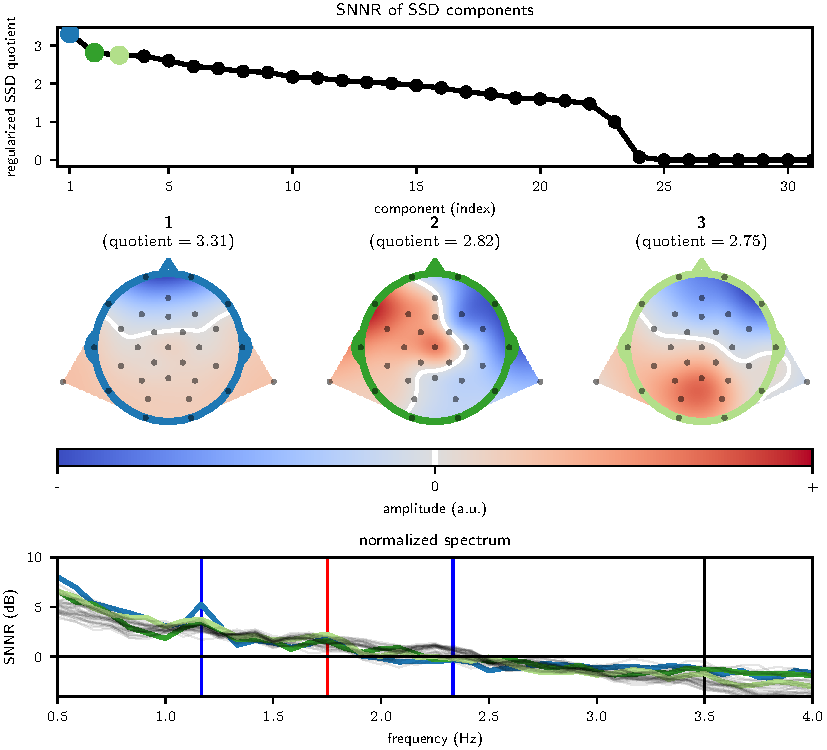
\includegraphics{./S01/FFTSSD_patterns}} & \tabcell{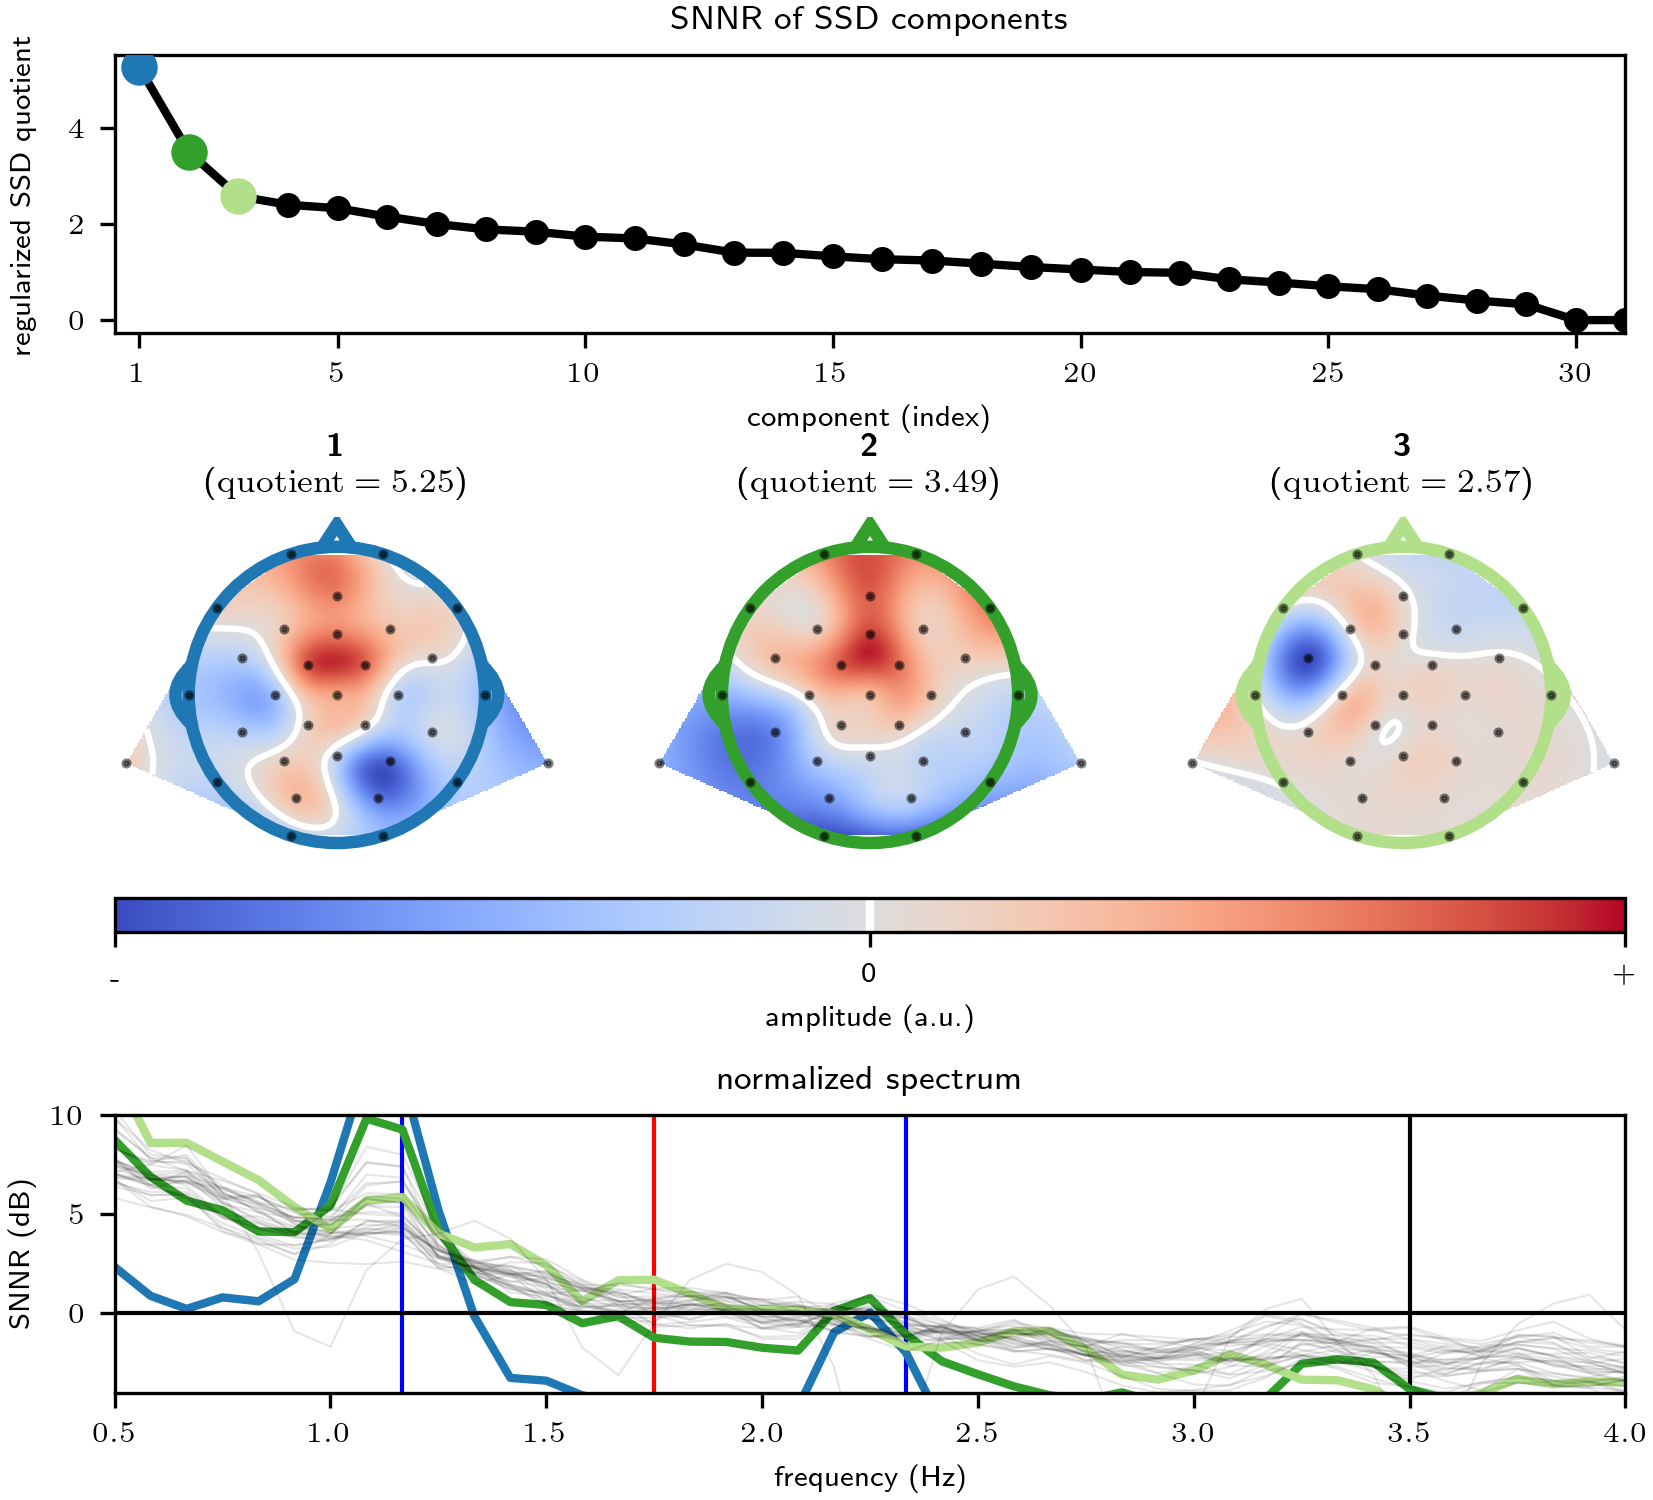
\includegraphics{./S02/FFTSSD_patterns}} & \tabcell{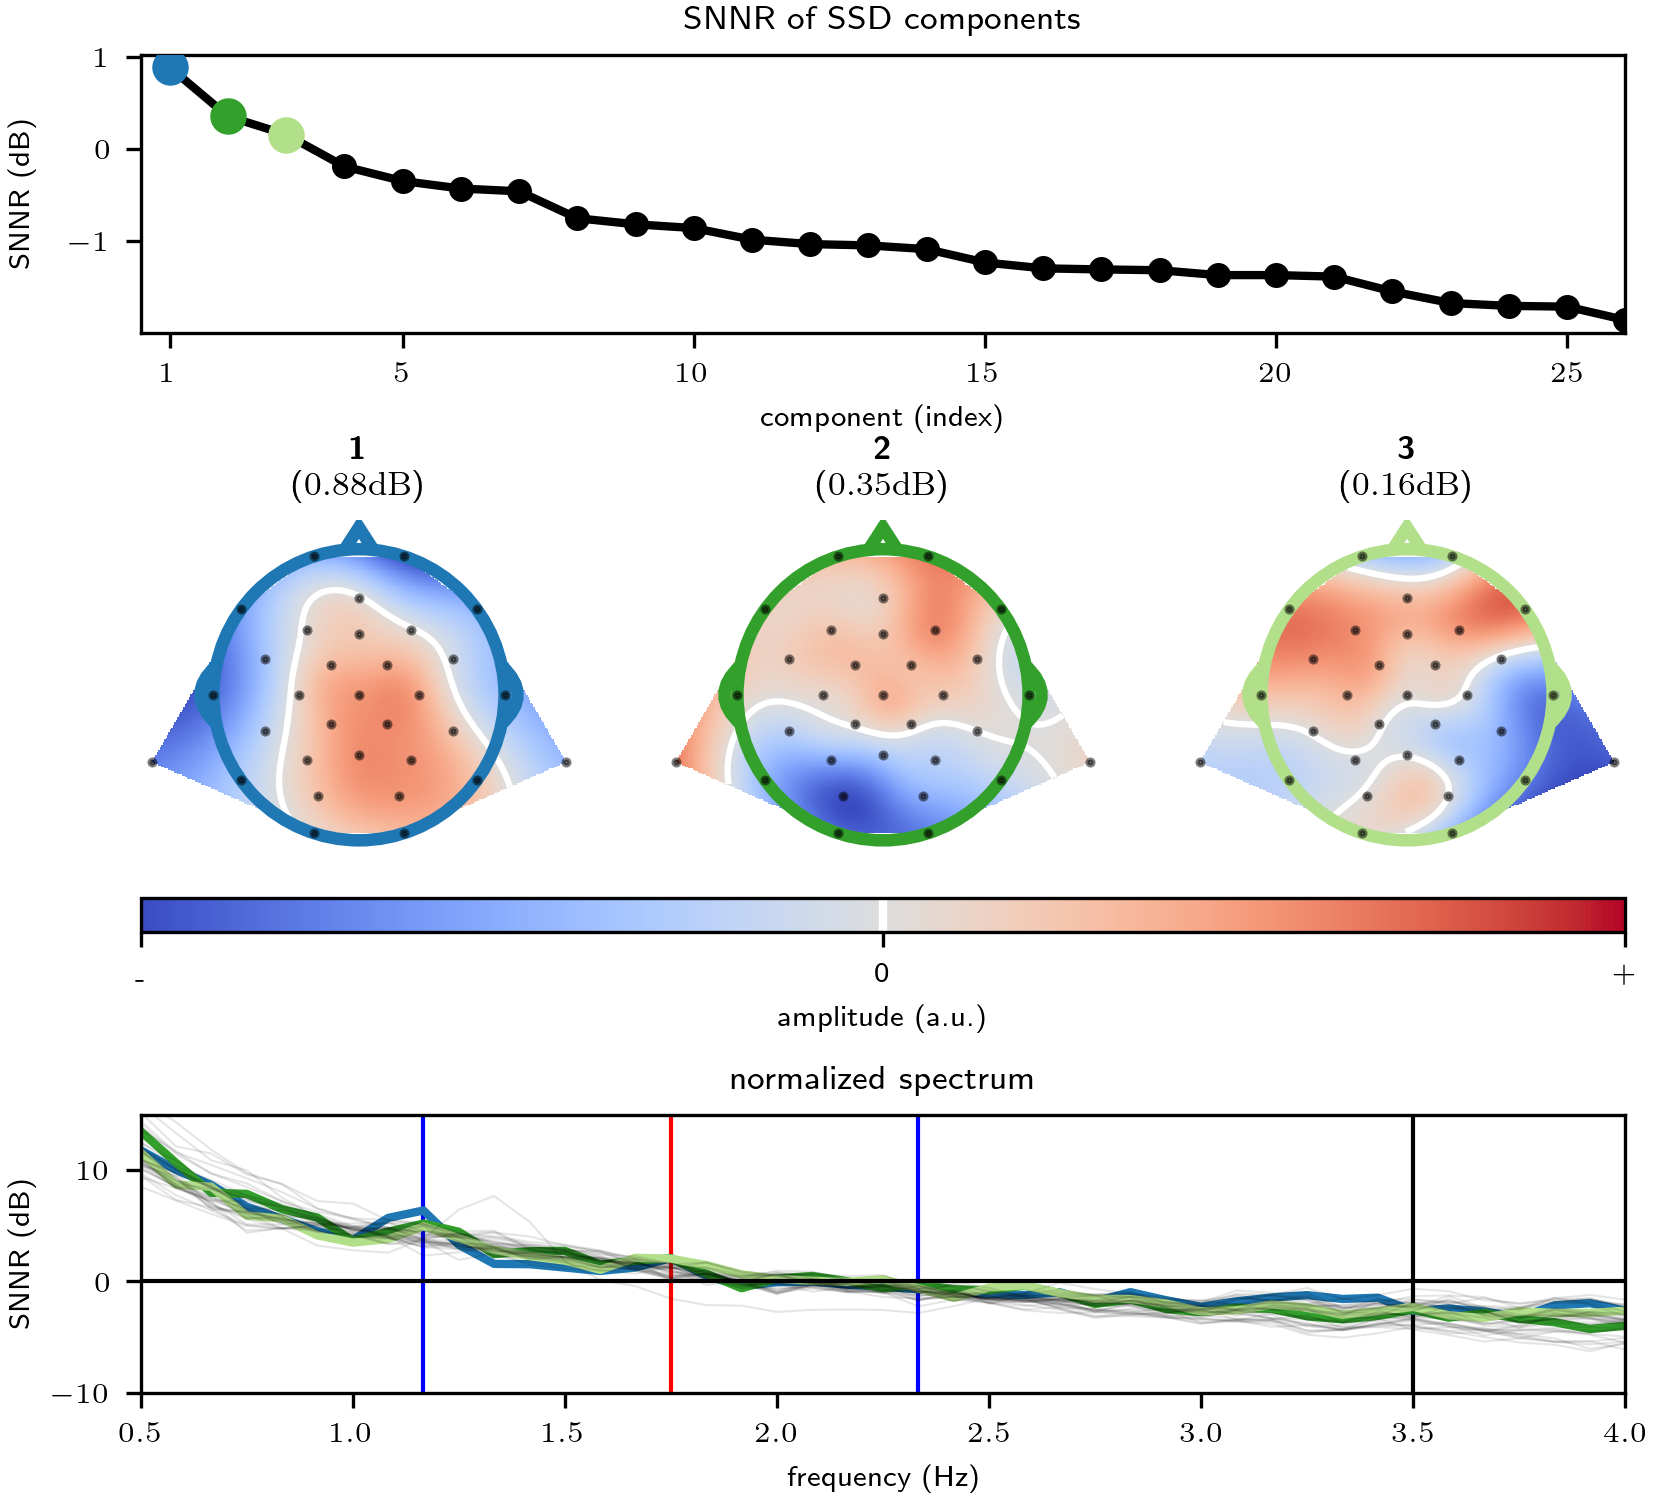
\includegraphics{./S03/FFTSSD_patterns}} & \tabcell{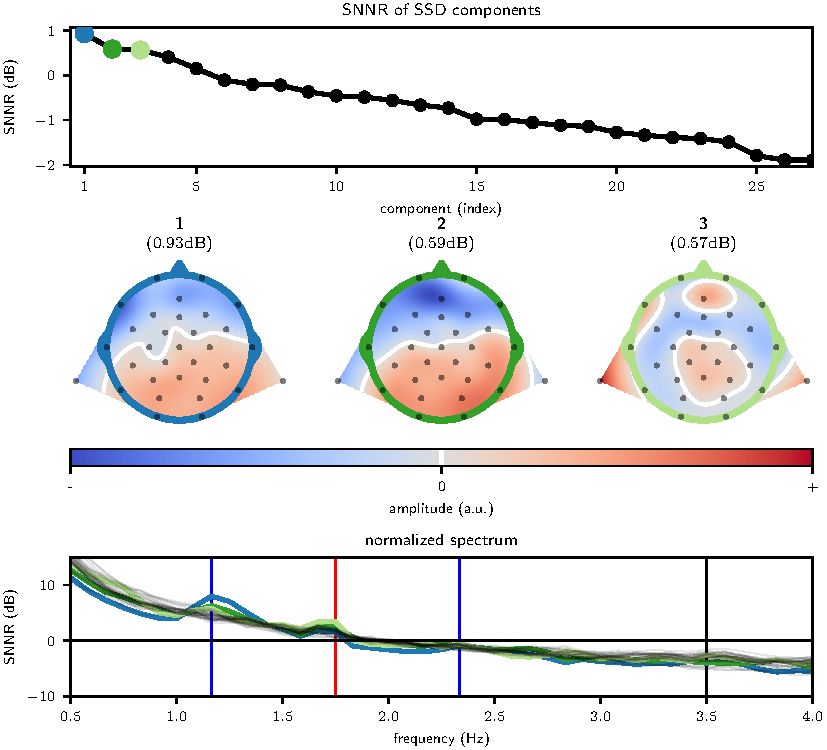
\includegraphics{./S04/FFTSSD_patterns}} \tabularnewline\midrule

	\tabcell{\textbf{S05}} & \tabcell{\textbf{S06}} & \tabcell{\textbf{S07}} & \tabcell{\textbf{S08}} \tabularnewline
        \tabcell{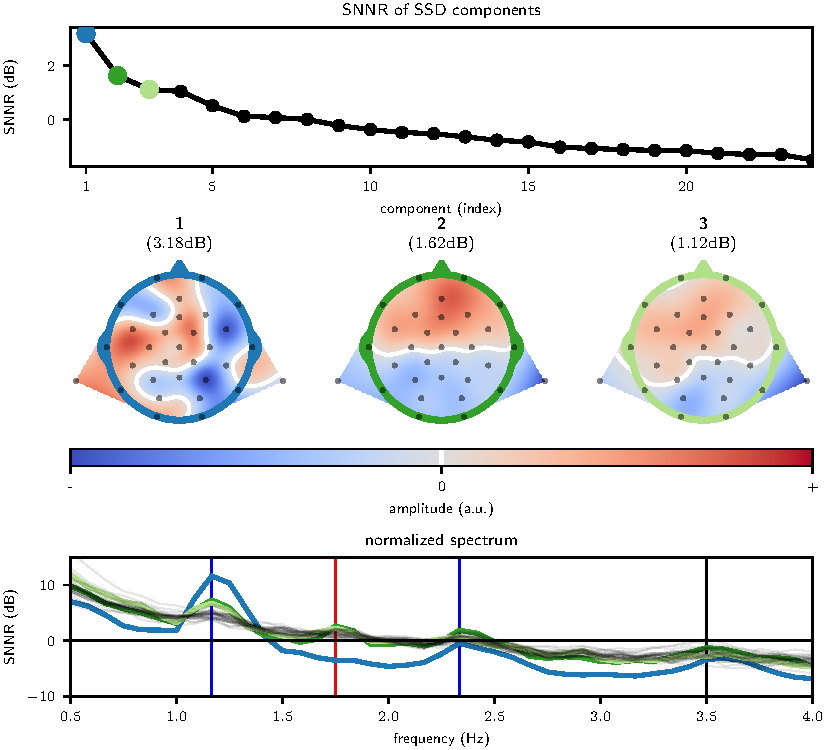
\includegraphics{./S05/FFTSSD_patterns}} & \tabcell{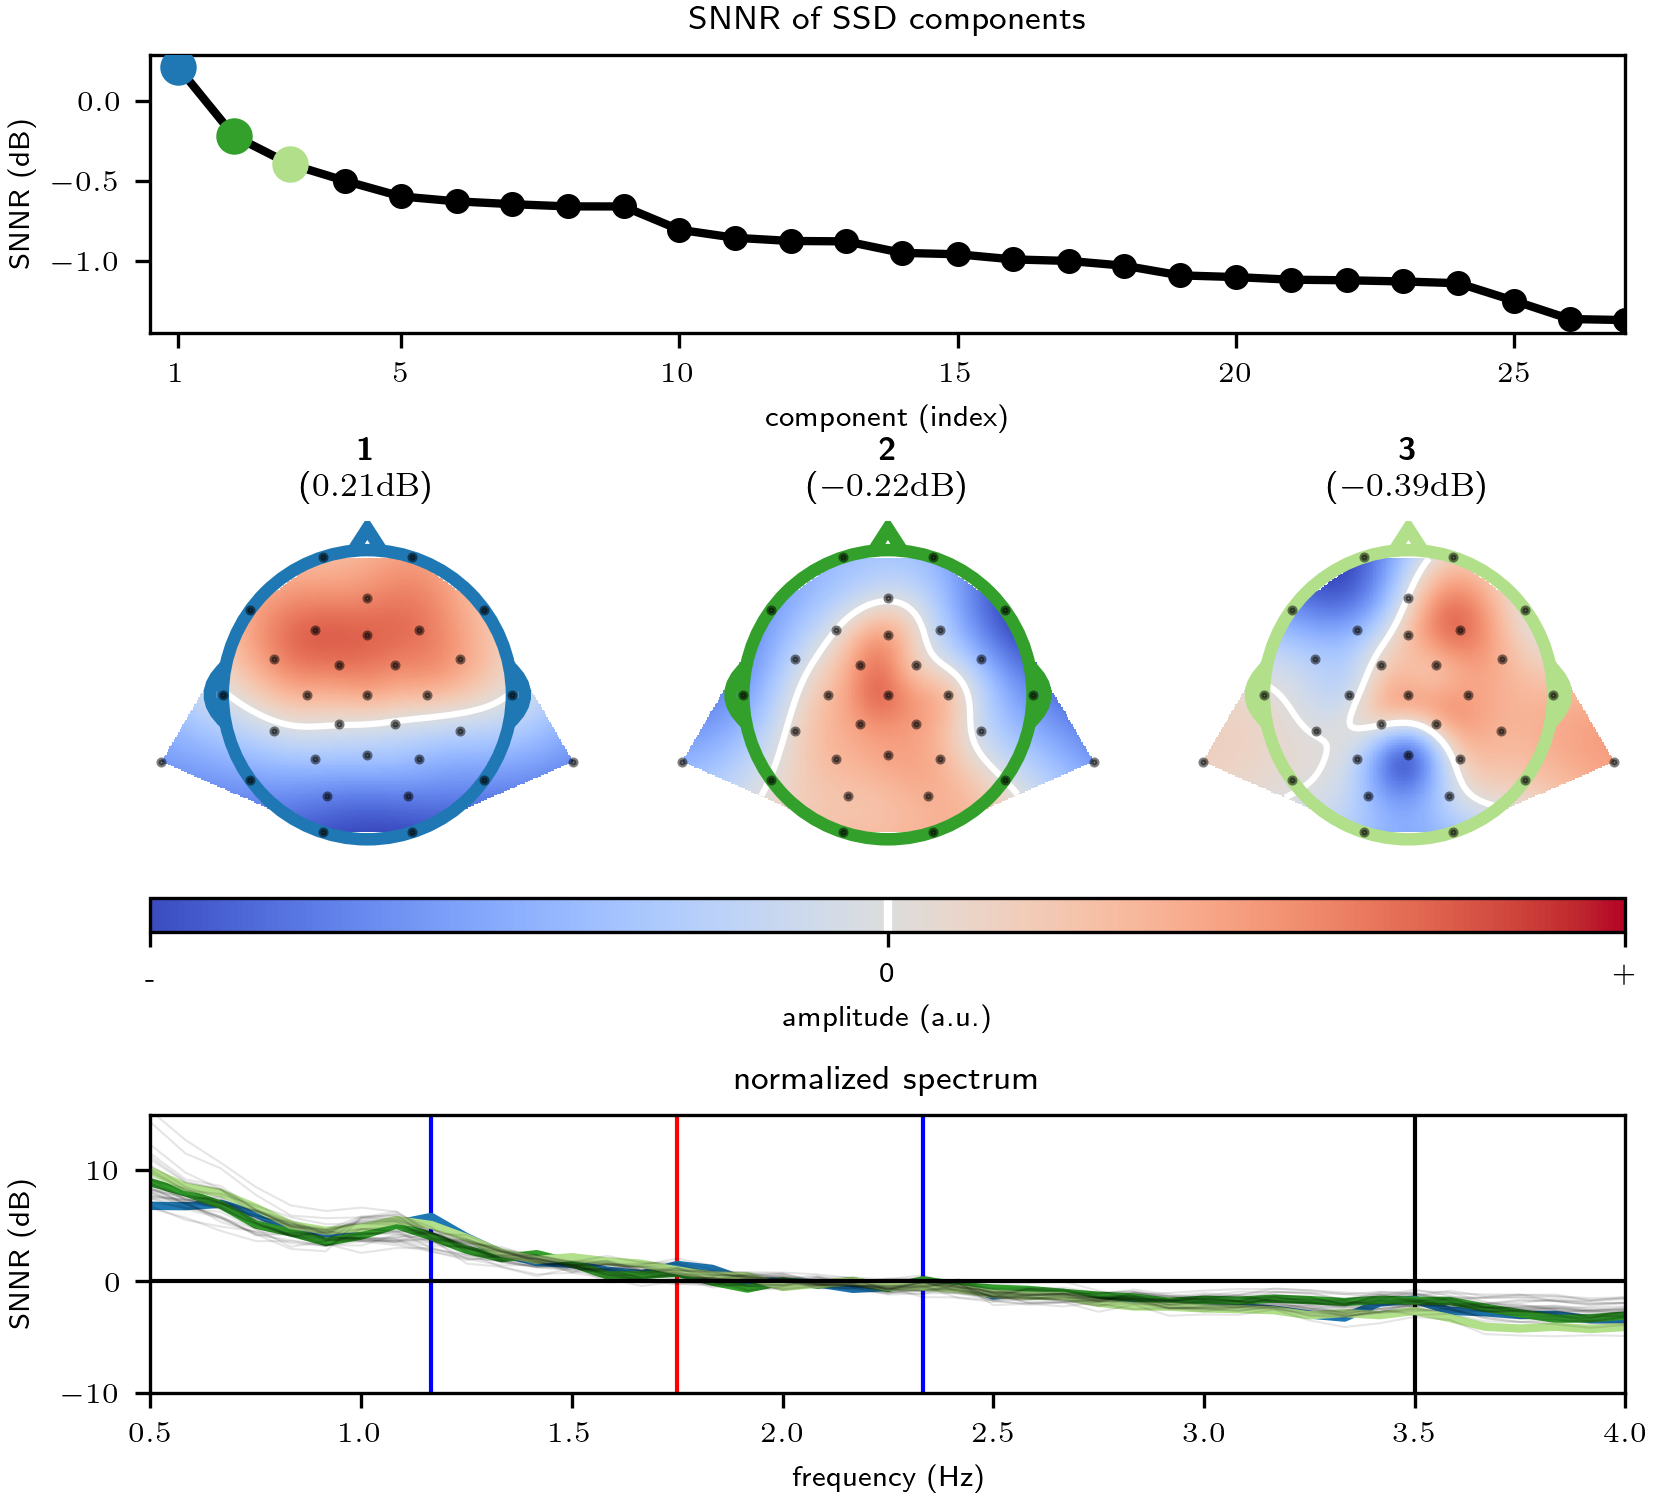
\includegraphics{./S06/FFTSSD_patterns}} & \tabcell{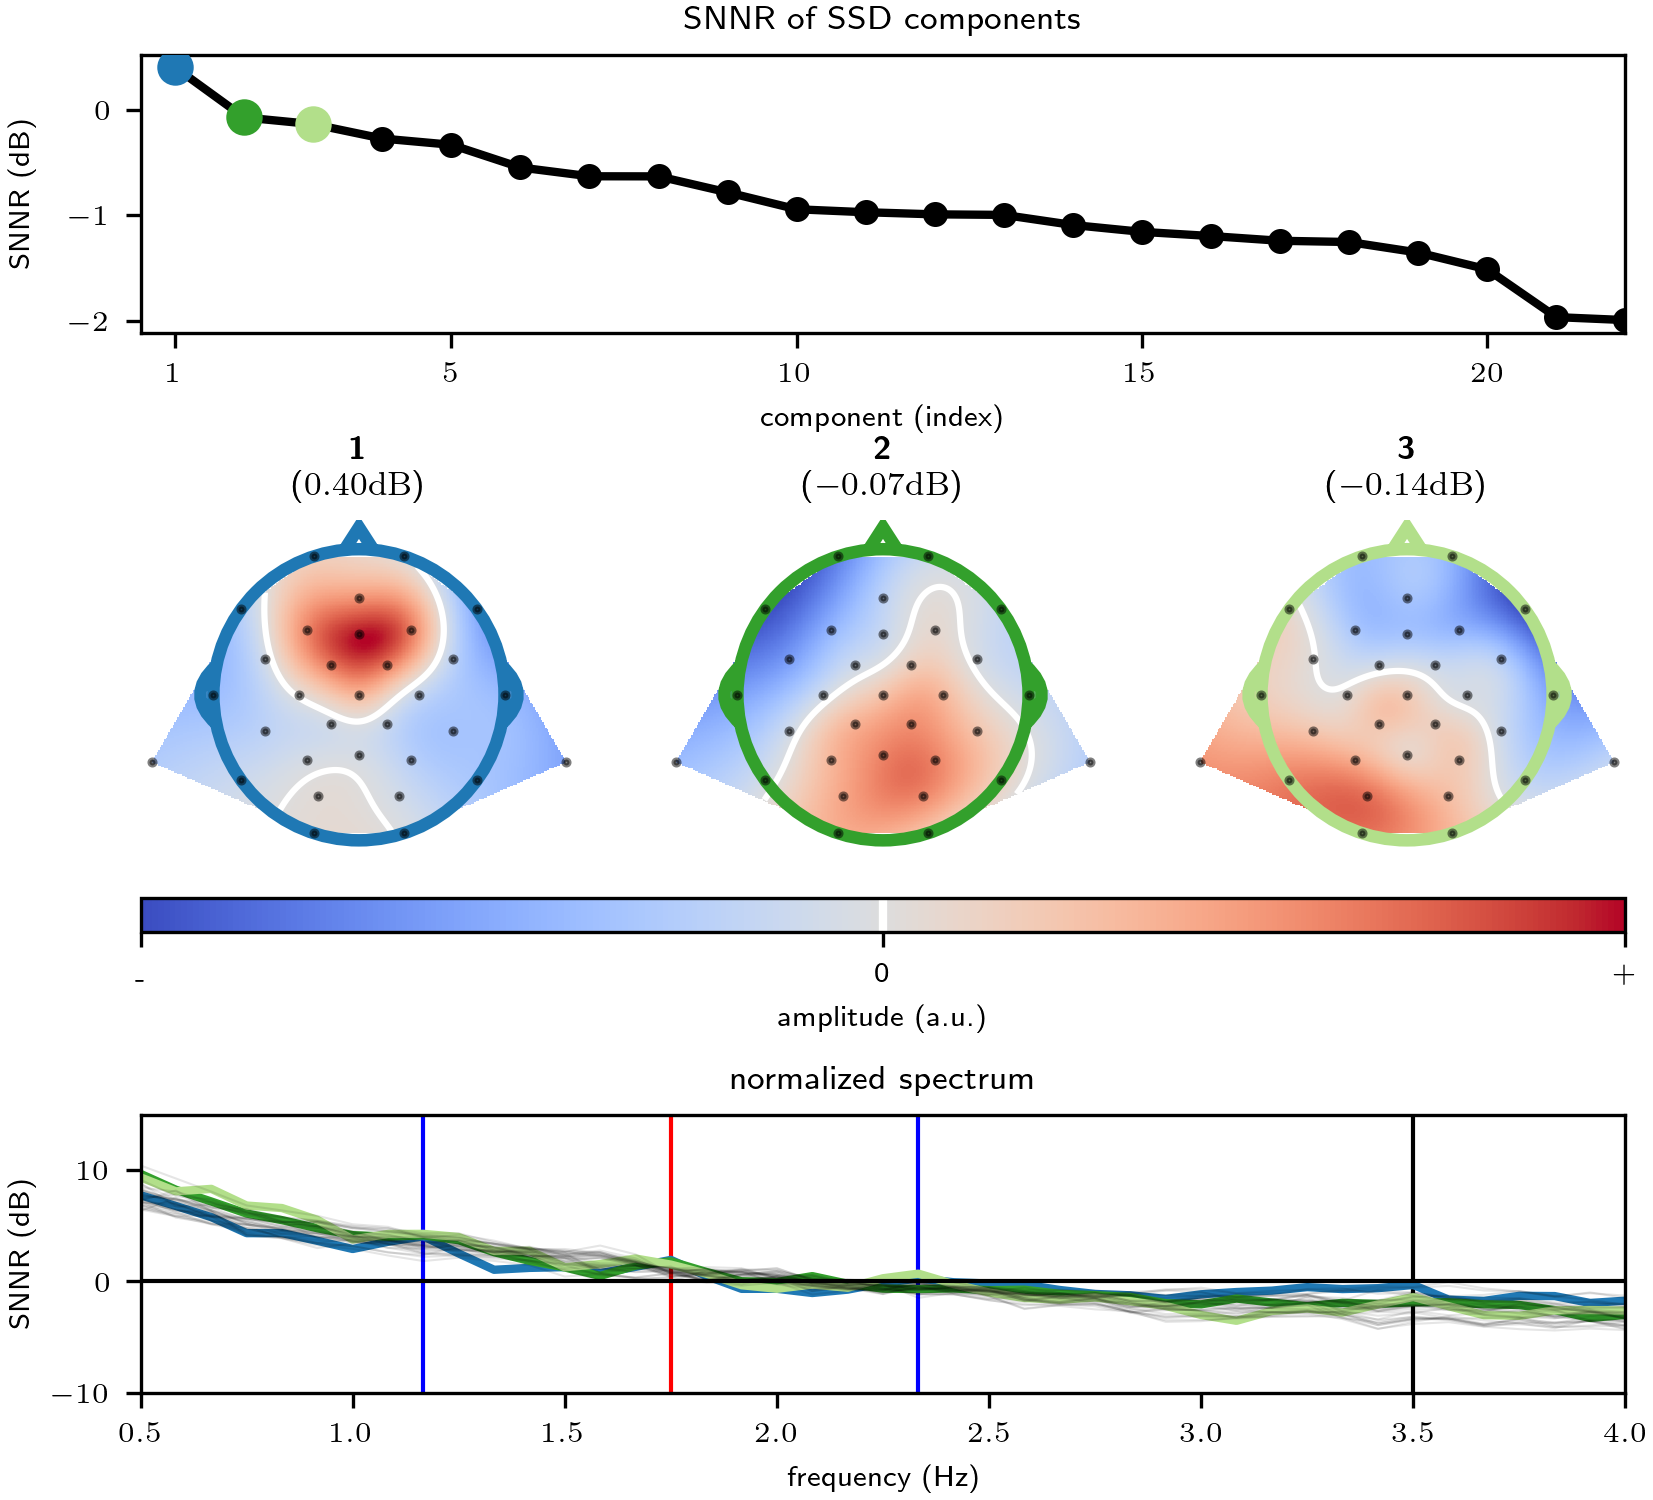
\includegraphics{./S07/FFTSSD_patterns}} & \tabcell{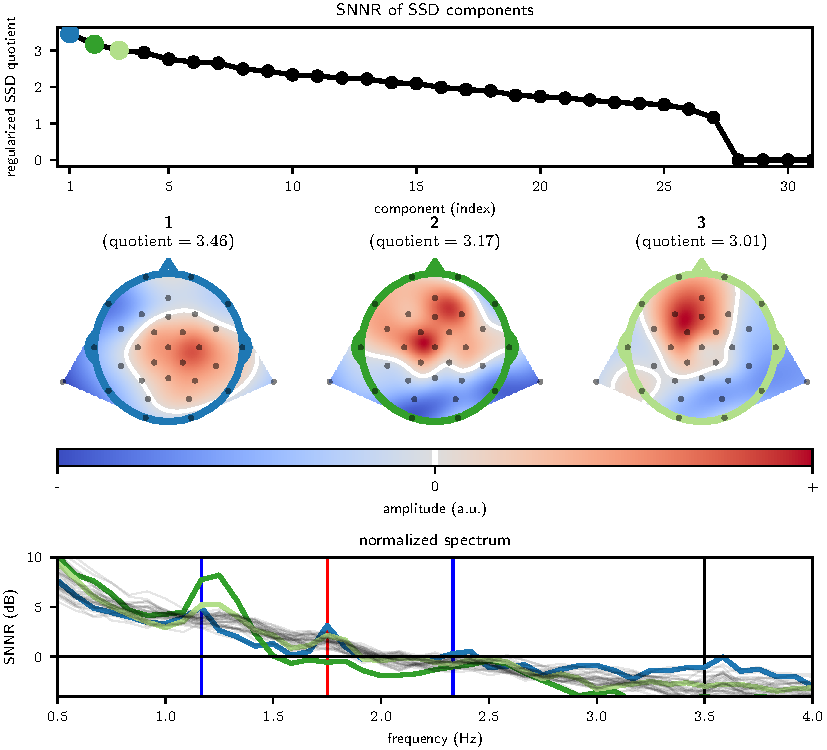
\includegraphics{./S08/FFTSSD_patterns}} \tabularnewline\midrule

	\tabcell{\textbf{S09}} & \tabcell{\textbf{S10}} & \tabcell{\textbf{S12}} & \tabcell{\textbf{S13}} \tabularnewline
        \tabcell{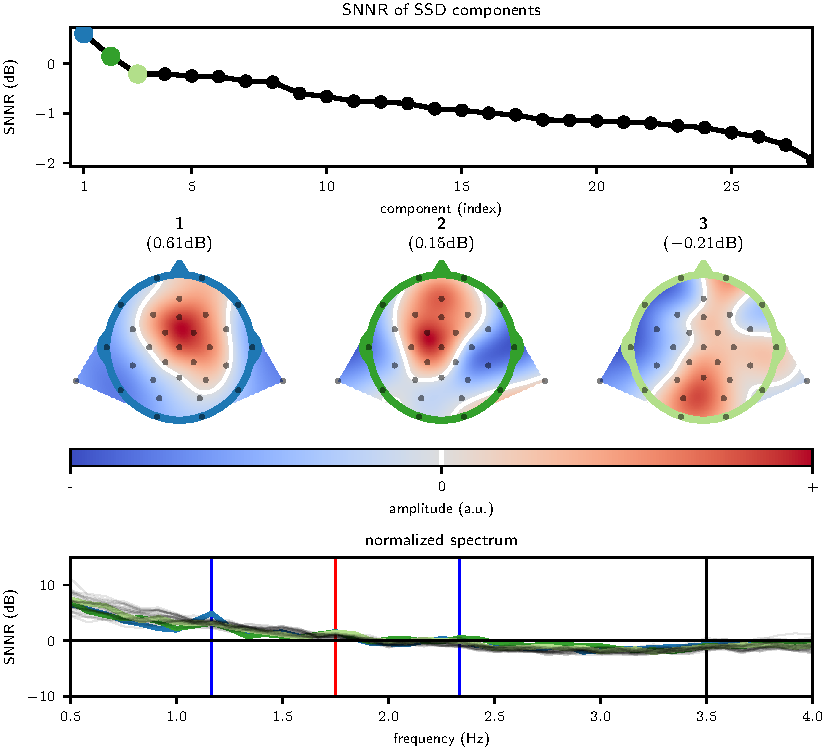
\includegraphics{./S09/FFTSSD_patterns}} & \tabcell{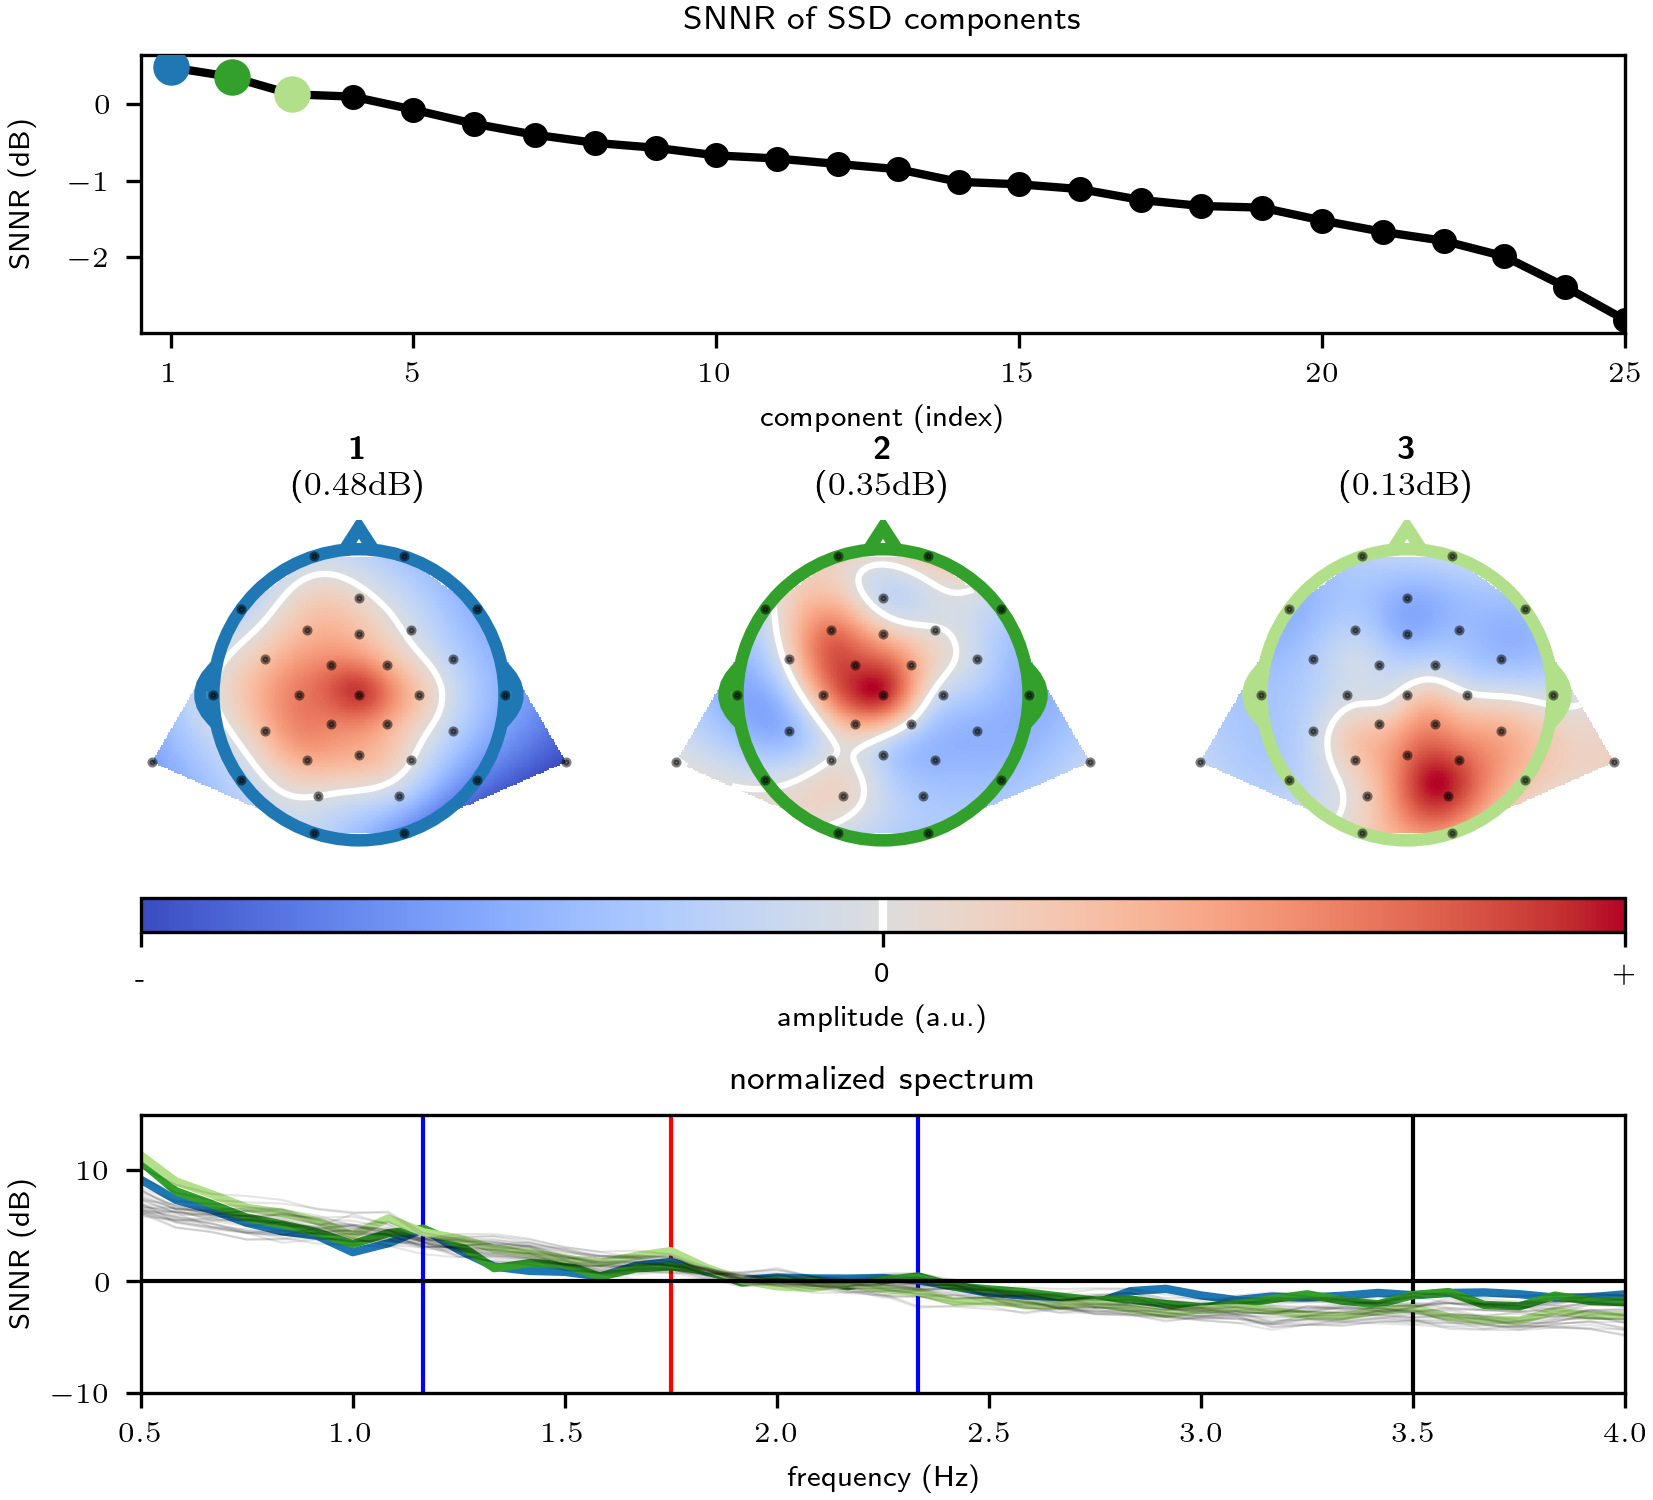
\includegraphics{./S10/FFTSSD_patterns}} & \tabcell{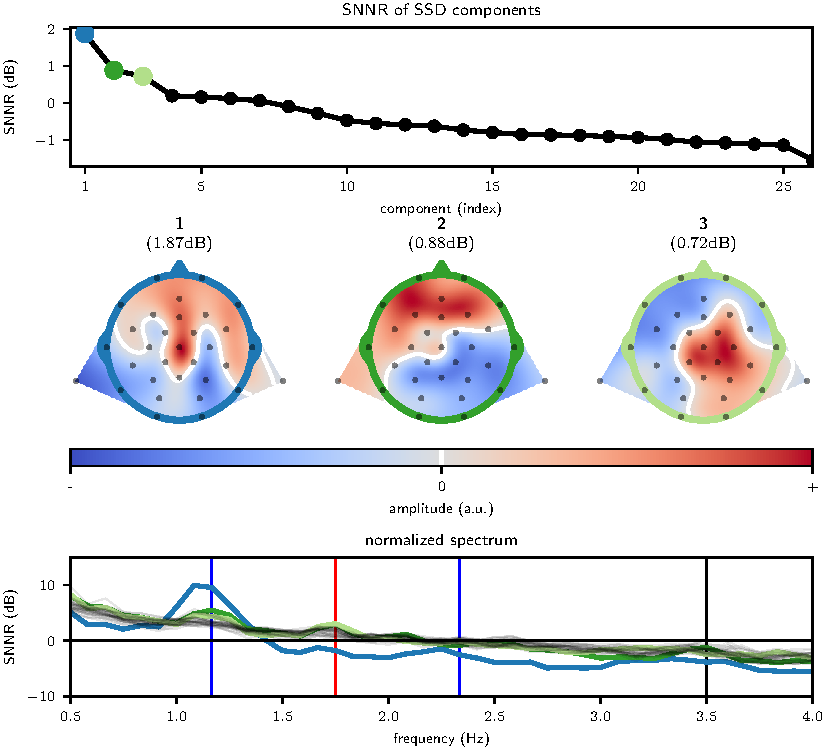
\includegraphics{./S12/FFTSSD_patterns}} & \tabcell{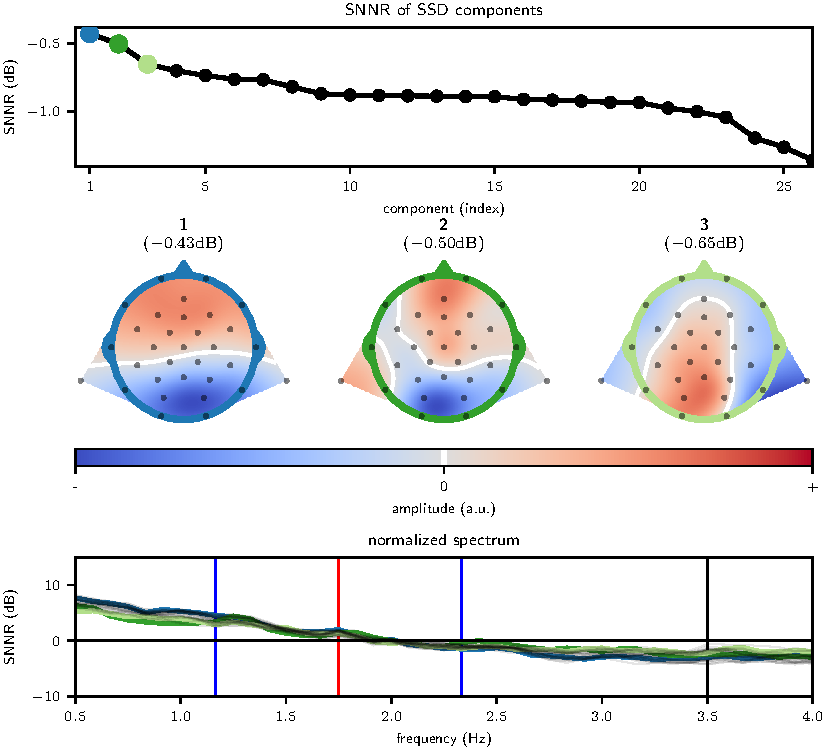
\includegraphics{./S13/FFTSSD_patterns}} \tabularnewline\midrule

	\tabcell{\textbf{S14}} & \tabcell{\textbf{S15}} & \tabcell{\textbf{S16}} & \tabcell{\textbf{S17}} \tabularnewline
        \tabcell{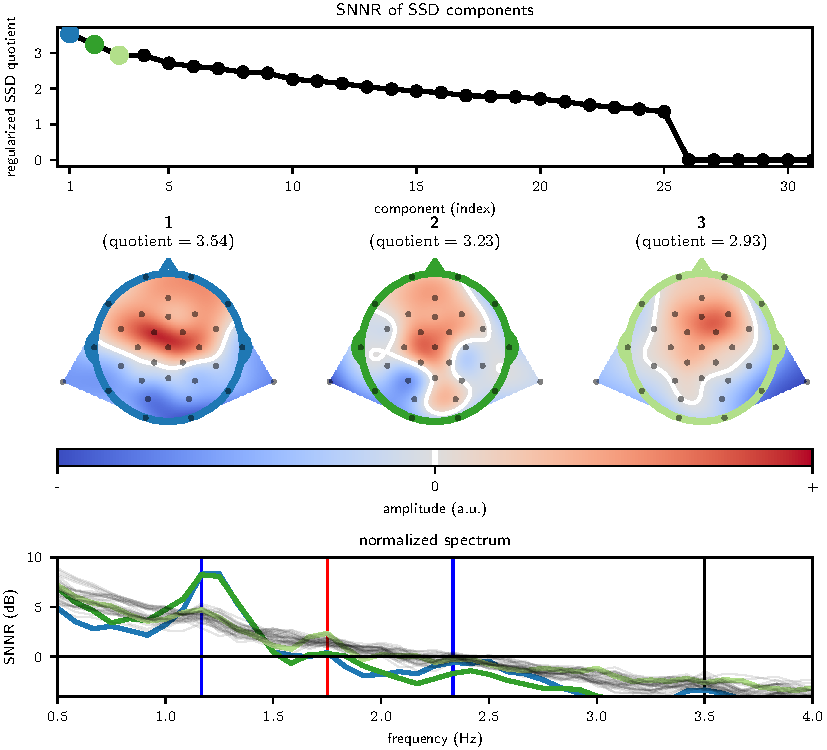
\includegraphics{./S14/FFTSSD_patterns}} & \tabcell{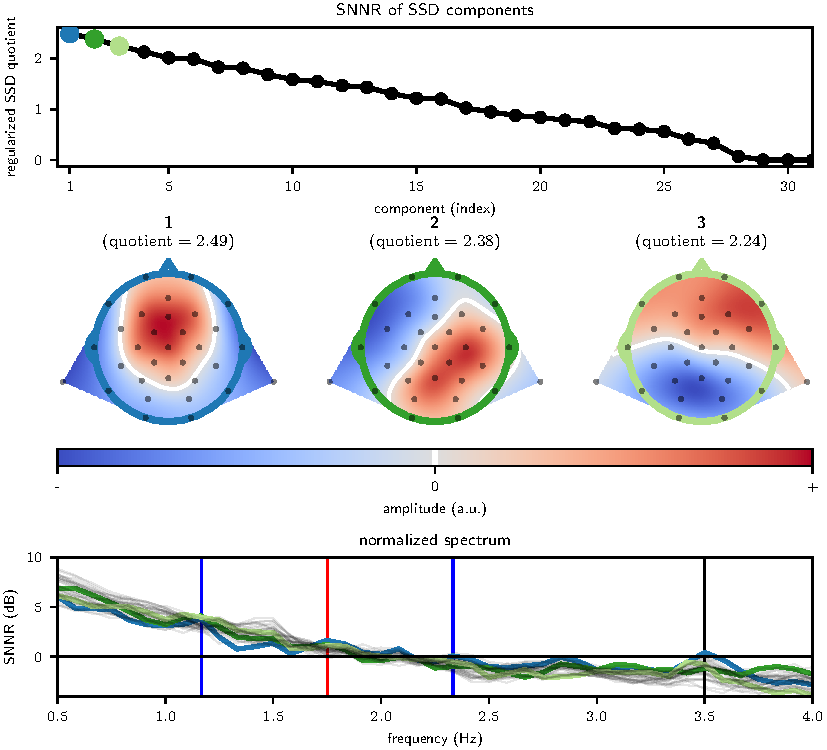
\includegraphics{./S15/FFTSSD_patterns}} & \tabcell{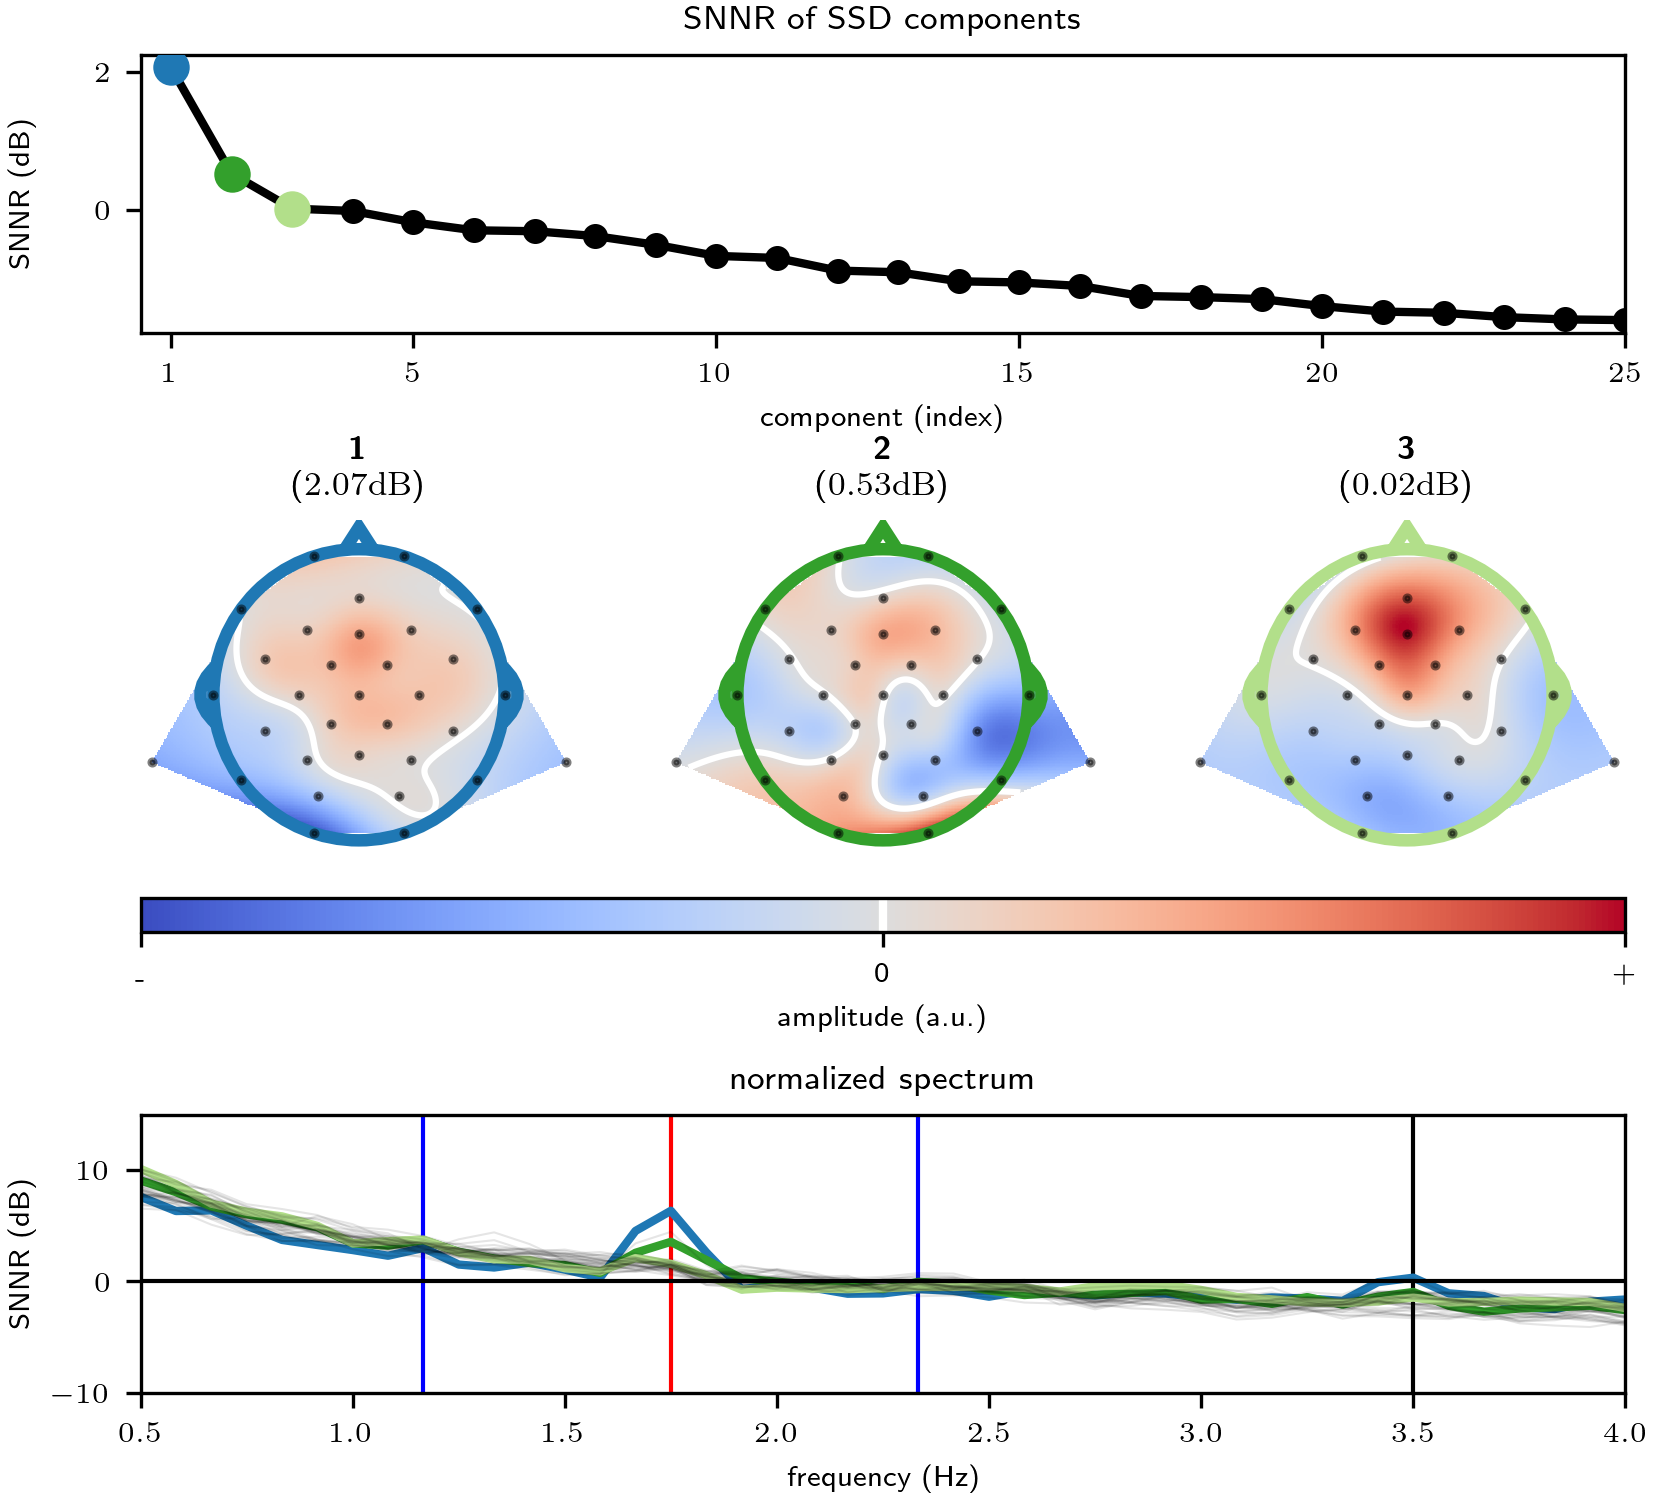
\includegraphics{./S16/FFTSSD_patterns}} & \tabcell{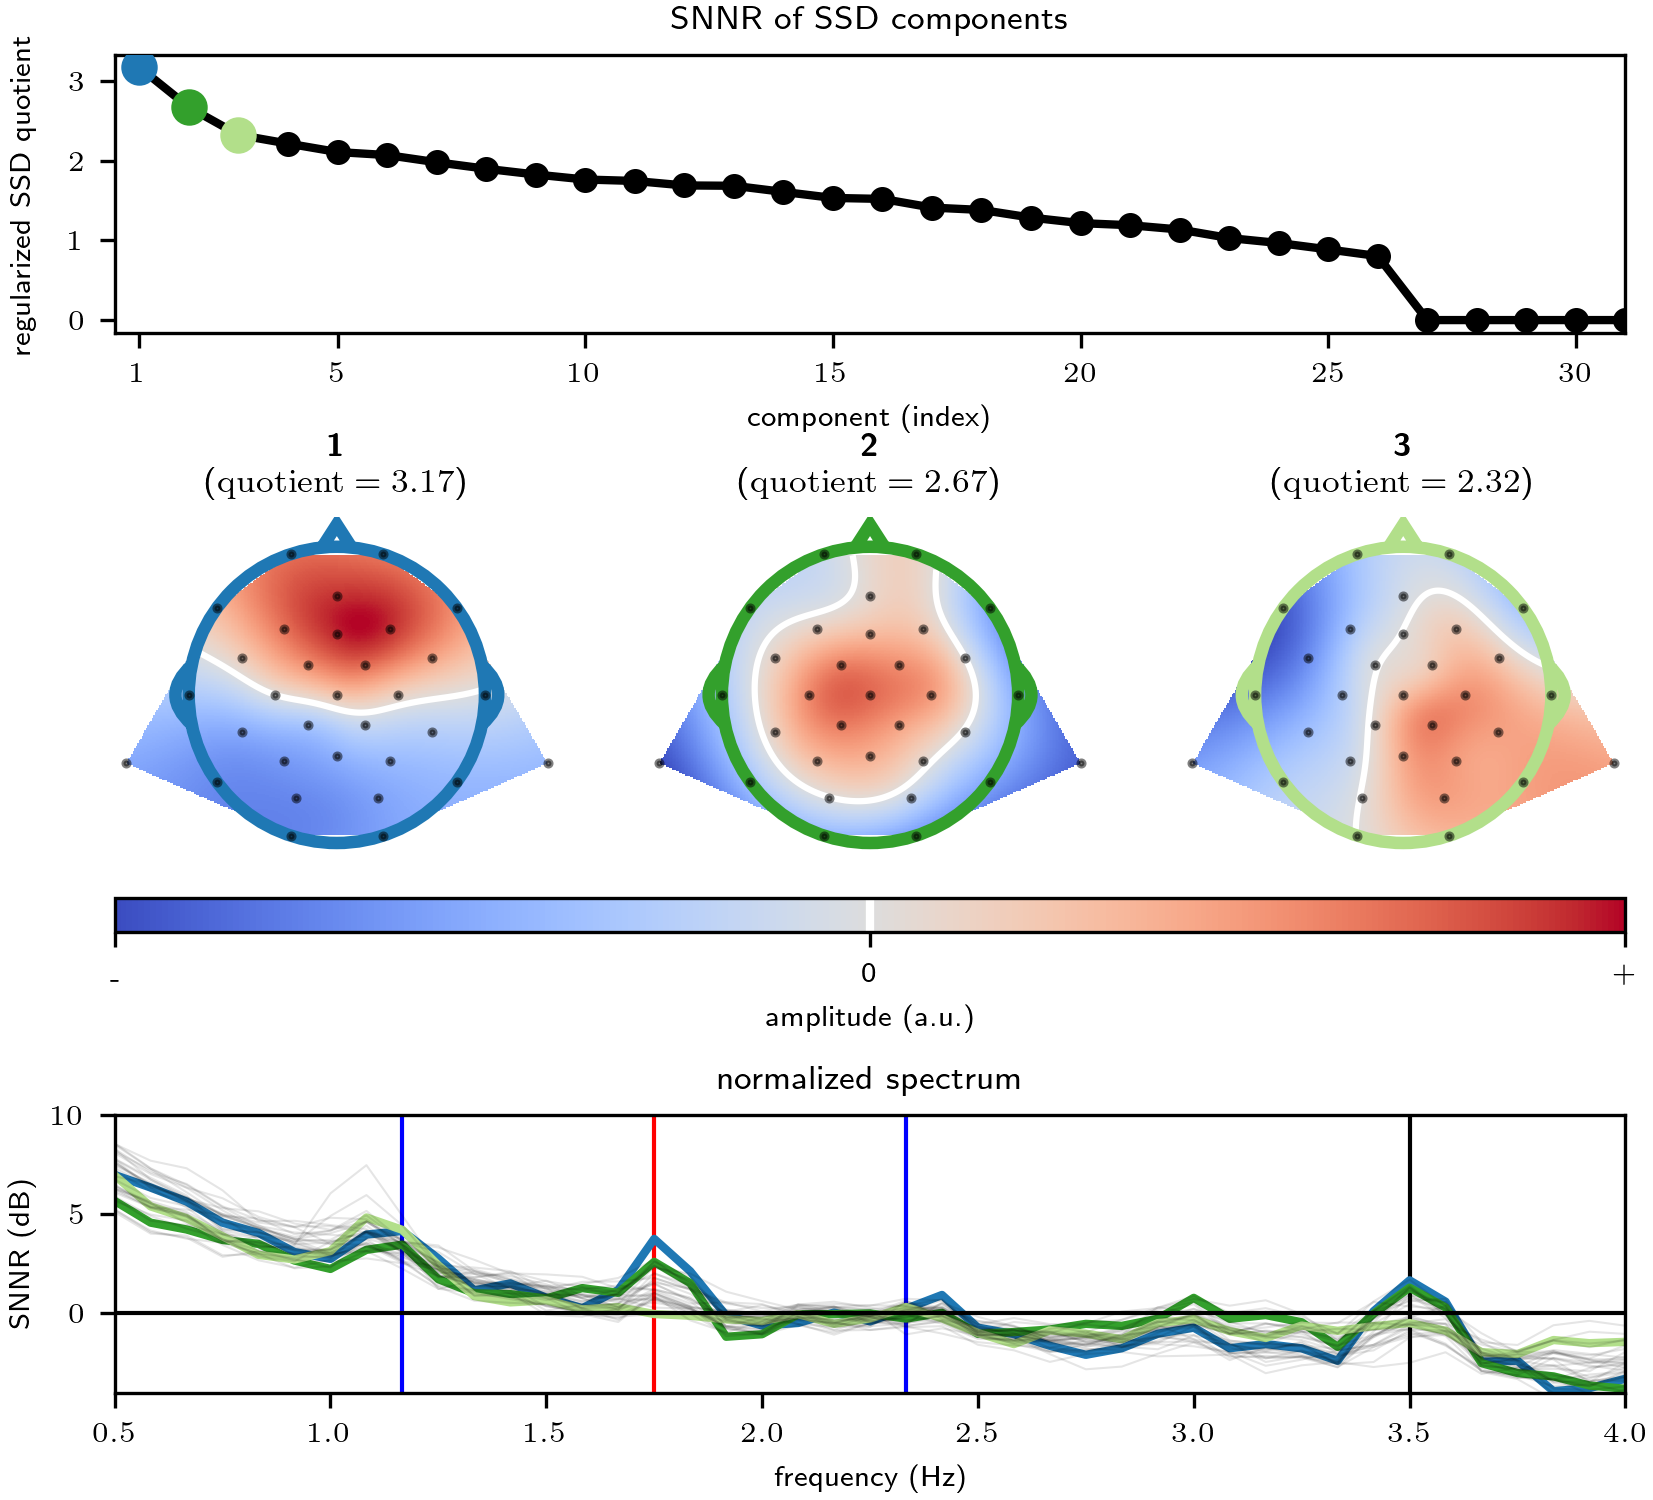
\includegraphics{./S17/FFTSSD_patterns}} \tabularnewline\midrule


	\tabcell{\textbf{S18}} & \tabcell{\textbf{S19}} & \tabcell{\textbf{S20}} & \tabcell{\textbf{S21}} \tabularnewline
        \tabcell{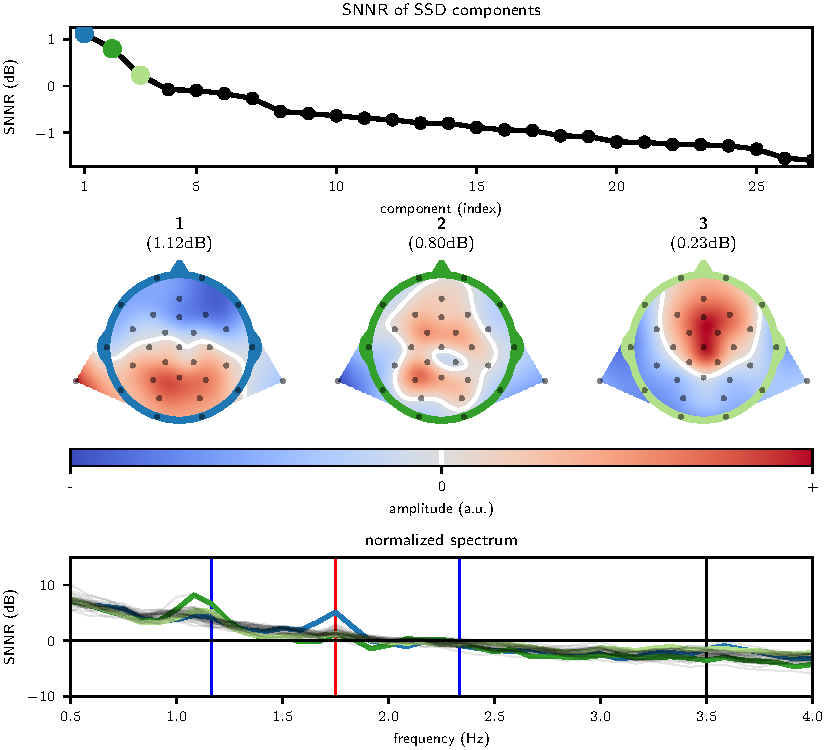
\includegraphics{./S18/FFTSSD_patterns}} & \tabcell{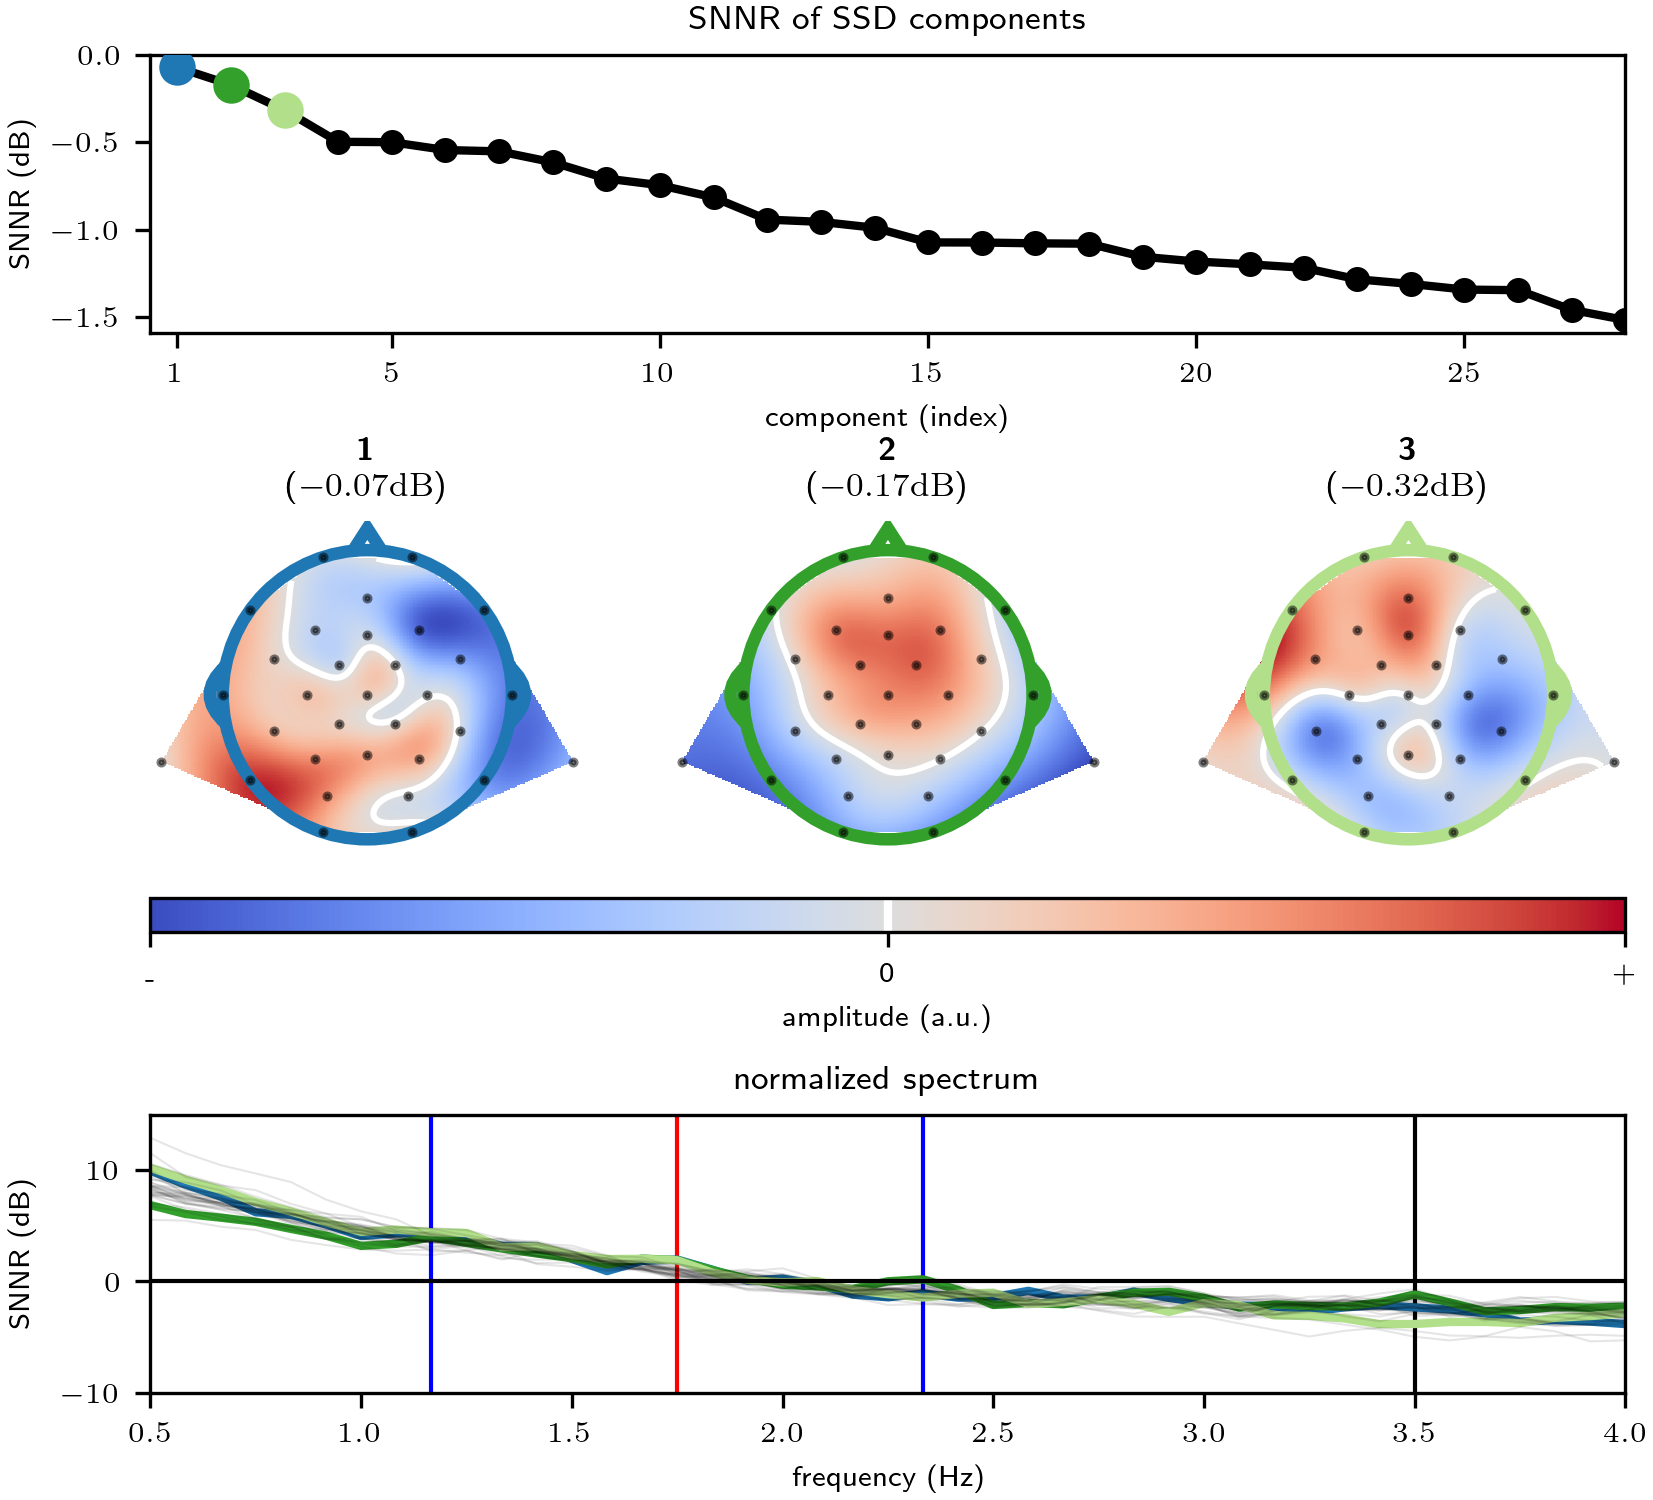
\includegraphics{./S19/FFTSSD_patterns}} & \tabcell{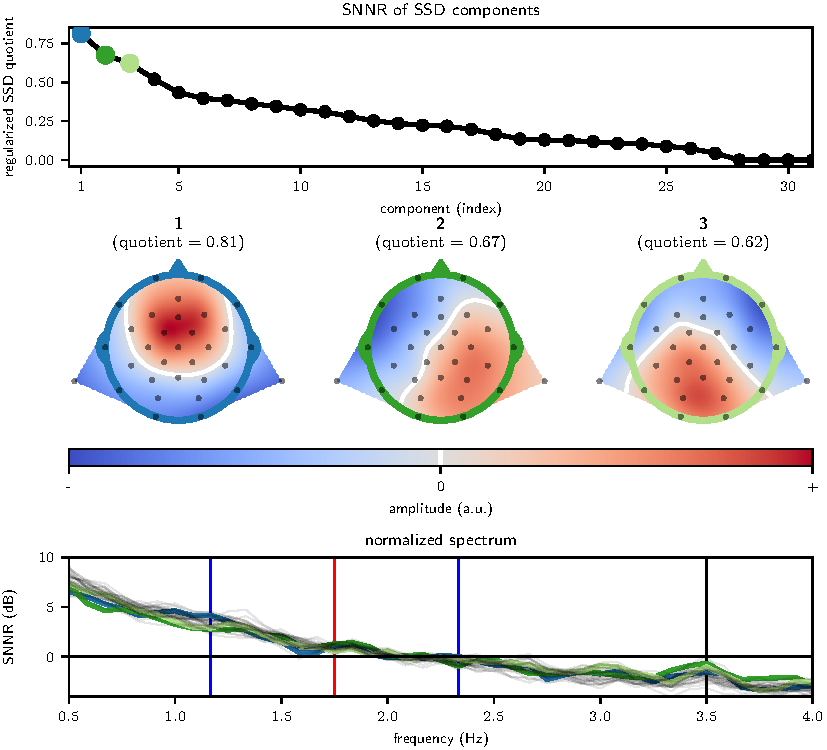
\includegraphics{./S20/FFTSSD_patterns}} & \tabcell{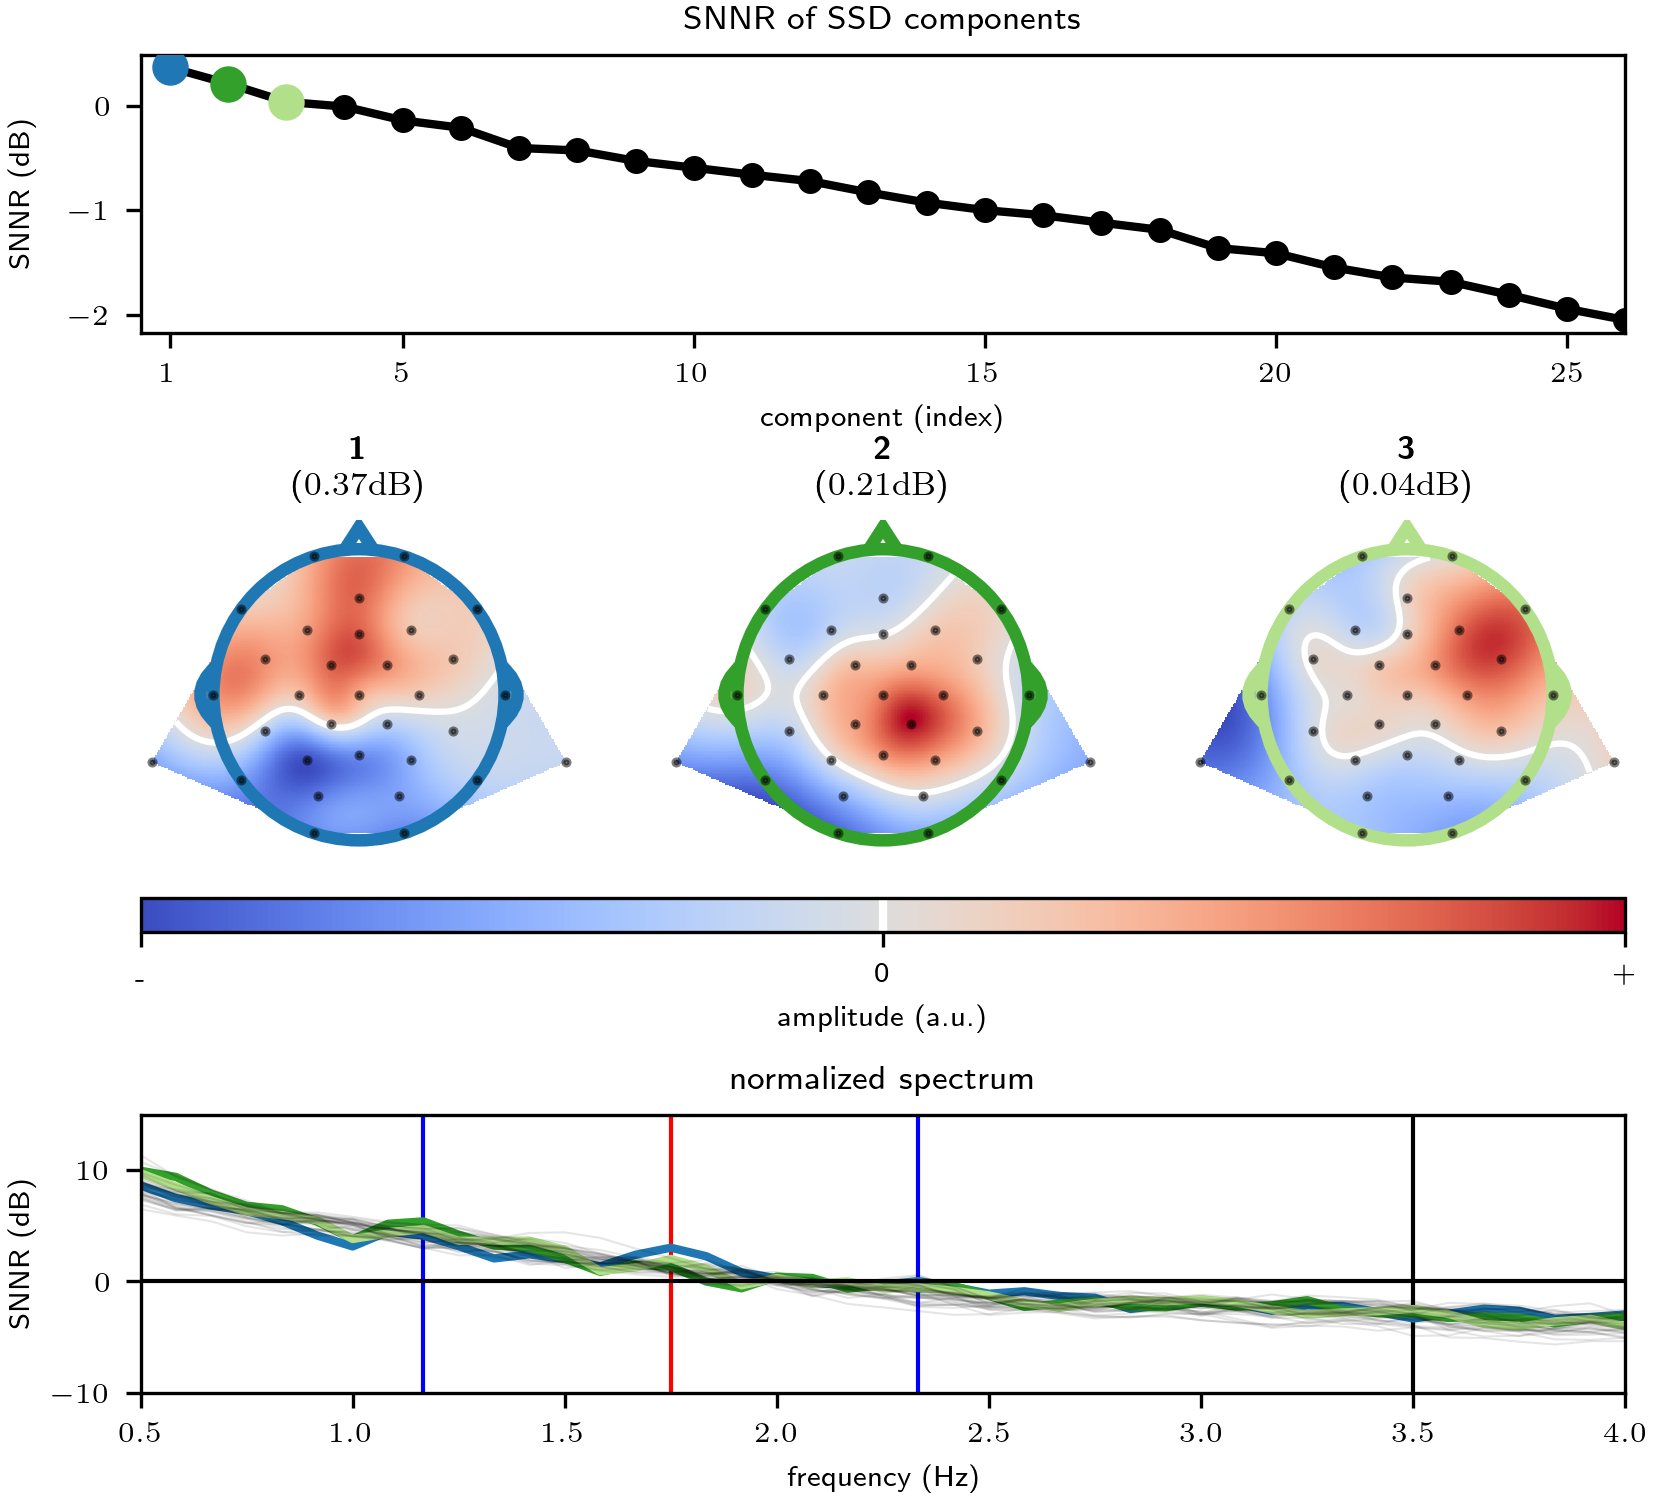
\includegraphics{./S21/FFTSSD_patterns}} \tabularnewline\bottomrule

\end{tabular}
\caption{xxx}
\end{threeparttable}

\end{document}
